\subsection{Definition}

\begin{figure}[!htb]
\begin{minipage}[t]{0.48\textwidth}
\vspace{-1.5cm}
We consider a 1D half-domain which is unlimited extended in one coordinate direction ($z\rightarrow\infty$).  
\end{minipage}
\hspace{0.02\textwidth}
\begin{minipage}[t]{0.48\textwidth}
\centering
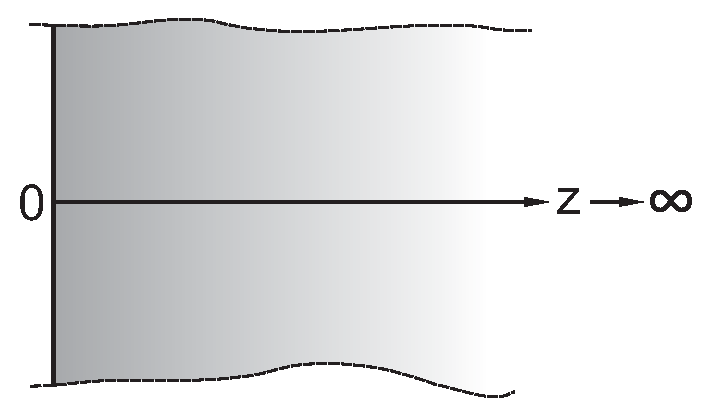
\includegraphics[scale=0.28]{PART_II/T/LHD.eps}
\caption{Model domain}
\label{fig:}
\end{minipage}
\end{figure}

\vspace{-1cm}

\subsection{Solution}
\subsubsection{Analytical solution}

The analytical solution for the 1D linear heat conduction equation (\ref{eqn:heat_conduction}) is
%\eqref{eqn:lhd}
\begin{equation}
T(x,t) = T_0 \operatorname{erfc} \left(\frac{x}{\sqrt{4\alpha t}}\right),
\label{eqn:lhd}
\end{equation}
where $T_0$ is the initial temperature. The boundary conditions are $T(z=0)=1$ and $T(z\rightarrow\infty)=0$.

The material properties for this model setup are given in Tab.~\ref{tab-ldhp}.

%\begin{table}[tab-ldhp]
%\centering
%\label{tab-ldhp}
%\caption{Material properties}
%\begin{tabular}{|c|l|l|}
%\hline
%symbol & quantity & value \\
%\hline
%$\rho$   & density of the solid & 2500  kg$\cdot$m$^{-3}$ \\			
%\hline
%$c$	     & thermal capacity	    & 1000  J$\cdot$kg$^{-1}\cdot$K$^{-1}$ \\
%\hline
%$\lambda$ & thermal conductivity	& 3.2  W$\cdot$m$^{-1}\cdot$K$^{-1}$ \\
%\hline
%\end{tabular}
%\end{table}
\begin{table}[h]%[tab-ldhp]
\caption{\label{tab-ldhp}Solid phase material properties}
\begin{center}
\begin{tabular}{llrr}
\toprule
Symbol & Parameter & Value & Unit \\
\midrule
$\rho$ & Density & 2500 & kg$\cdot$m$^{-3}$ \\			
$c$	   & Heat capacity & 1000 & J$\cdot$kg$^{-1}\cdot$K$^{-1}$ \\
$\lambda$	& Thermal conductivity & 3.2 & W$\cdot$m$^{-1}\cdot$K$^{-1}$ \\
\bottomrule
\end{tabular}
\end{center}
\end{table}

Using these values, the heat diffusivity constant is $\alpha = \lambda/c\rho = 1.28 \cdot 10^{-6}m^2/s$.

\subsubsection{Numerical solution}

The numerical model consists of 60 line elements connected by 61 nodes along the z-axis (figure \ref{fig-ms-lhd}). The distances of the nodes $\Delta z$ is one meter. At $z=\unit[0]{m}$ there is a constant temperature boundary condition. 

\begin{figure}%[img-msldh]
%\label{img-msldh}
\centering
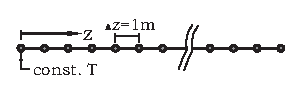
\includegraphics[width=0.5\textwidth]{PART_II/T/ms-lhd.eps}
\caption{\label{fig-ms-lhd}Spatial discretisation of the numerical model}
\end{figure}

The \textit{Neumann} stability criteria has to be restrained so that the temperature gradient can not be inverted by diffusive fluxes. Using \eqref{eqn:ne-ldh} the best time step can be estimated by
%
\begin{equation}
\operatorname{Ne} = \frac{\alpha\Delta t}{(\Delta z)^2}\leq\frac{1}{2}.
\label{eqn:ne-ldh}
\end{equation}
%
With $\Delta z=\unit[1]{m}$ and $\alpha=\unit[1.28 \cdot 10^{-6}]{m^2/s}$ the outcome for the timestep is $\Delta t\leq \unit[390625]{s}$ or 4.5 days, respectively.

\begin{figure}[htb!]%[img-lhd-all]
\centering
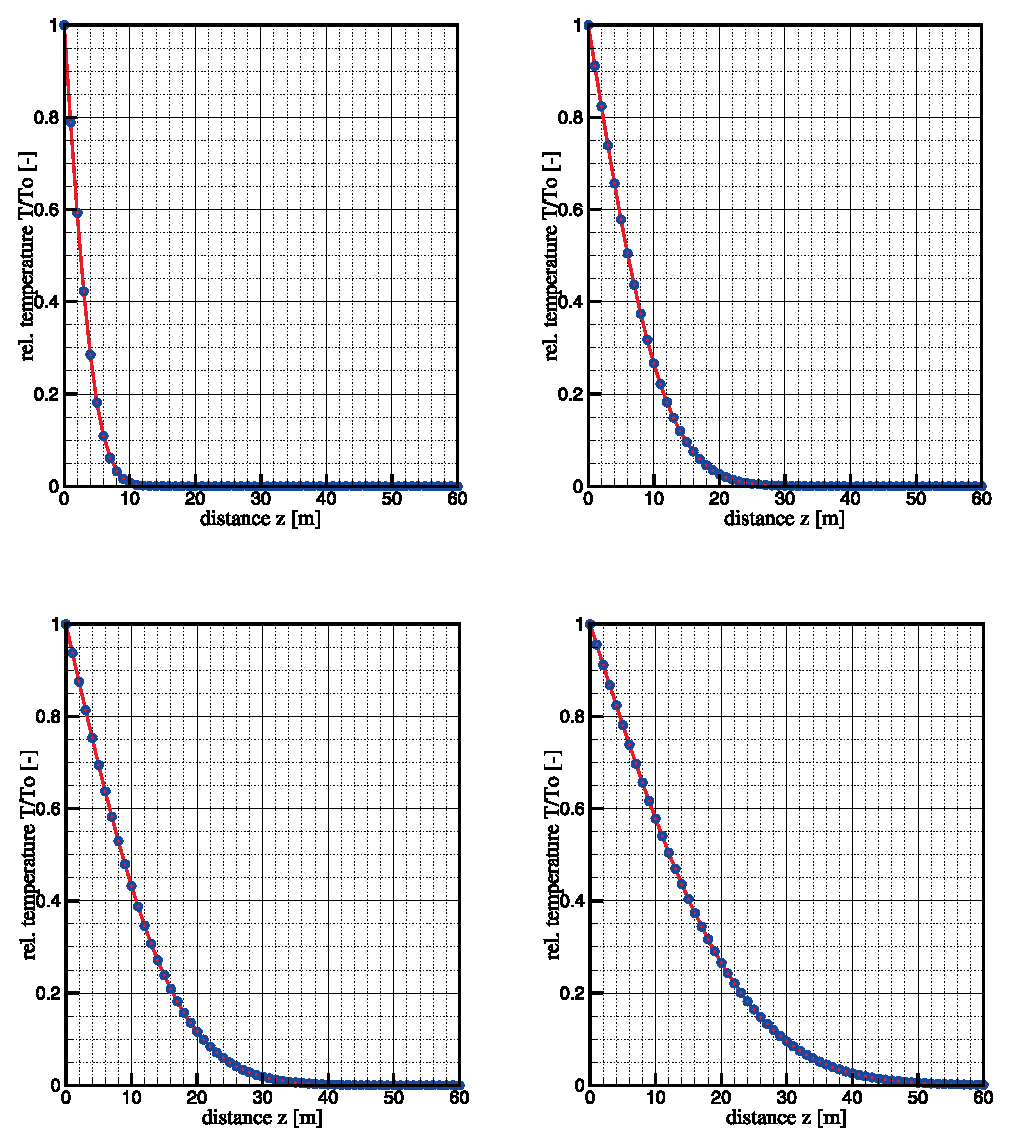
\includegraphics[width=0.9\textwidth]{PART_II/T/lhd-all.eps}
\caption{\label{fig-lhd-all}Temperature distribution along the z-axis after 2 months, 1 year, 2 years and 4 years (from top left to down right).}
\end{figure}

\subsection{Results}

%The following figure show the comparison of the solution of \eqref{eqn:lhd} and the numerical simulation results. Fig.~\ref{fig-lhd-all} shows the temperature distribution along the model domain after 2 months, 1 year, 2 years and 4 years.
Figures ~\ref{fig-lhd-all} show the comparison of the solution of \eqref{eqn:lhd} and the numerical simulation results. It is demontrated the temperature distribution along the model domain after 2 months, 1 year, 2 years and 4 years.

%\clearpage